%!TEX root = ../template.tex
%%%%%%%%%%%%%%%%%%%%%%%%%%%%%%%%%%%%%%%%%%%%%%%%%%%%%%%%%%%%%%%%%%%
%% chapter1.tex
%% NOVA thesis document file
%%
%% Chapter with introduction
%%%%%%%%%%%%%%%%%%%%%%%%%%%%%%%%%%%%%%%%%%%%%%%%%%%%%%%%%%%%%%%%%%%

\typeout{NT FILE chapter1.tex}%

\chapter{Introduction}
\label{cha:introduction}

\prependtographicspath{{Chapters/Figures/Covers/}}

% epigraph configuration
\epigraphfontsize{\small\itshape}
\setlength\epigraphwidth{12.5cm}
\setlength\epigraphrule{0pt}


\epigraph{
  This work is licensed under the \href{https://www.latex-project.org/lppl/lppl-1-3c/}{\LaTeX\ Project Public License v1.3c}.
  To view a copy of this \ntindex[Template!]{license}, visit the \href{https://www.latex-project.org/lppl/}{LaTeX project public license}.
}

\section{Multiscalar diagnostics in turbulent flames}
\label{sec:multiscalar_diagnostics}

This first Chapter introduces the \gls{novathesis} template and how it is organized. In Chapter~\ref{cha:users_manual} you can find some specific instructions on how to use this template.  Chapter~\ref{cha:a_short_latex_tutorial_with_examples} shows some examples and give some hints on how to write your text. Please read these next Chapters carefully.

\subsection{Your Time is Precious}
\label{sub:time_is_money}

Did you learn how to drive by sitting by the wheel and throwing your car into the road?  Most probably you did take your time \textit{learning the rules} and \emph{practicing} first! Likewise, it is not wise to throw yourself at the task of writing a thesis/dissertation in \LaTeX\ without seriously considering the following \ntindex{recommendation}!

\begin{tcolorbox}[colback=green!8]
  If you are going to spend zillions of hours writing your thesis/dissertation using the \gls{novathesis} \LaTeX\ template (or some other \LaTeX\ template), be wise and spend a couple of hours learning how to use it properly by reading its manual.  And then, be even wiser, and spend a few more hours \href{https://github.com/joaomlourenco/novathesis/wiki\#learning-latex}{learning some \LaTeX}.  I am sure that the time you are investing now will pay itself countless times before you submit your thesis/dissertation.\\\parbox{\linewidth}{\raggedleft---~\emph{João Lourenço}}
\end{tcolorbox}

\subsection{Recognition}
\label{sub:recognition}

\ntindex[Recognition]{}

The s} and:
\begin{enumerate}
  \item \ntindex[novathesis!Citation]{} Cite the \gls{novathesis} manual~\cite{novathesis-manual} in a place of your choice (e.g., in the \emph{Acknowledgments}) of your thesis/dissertation with “\verb!\cite{novathesis-manual}!” .  If you cite it this way, the correct entry will be added automatically to your bibliography (no need to worry with the necessary BibTeX entry, as it will be added automatically);
  \item Go to the
\href{https://github.com/joaomlourenco/novathesis}{\ntindex[GitHub!project web page]{project web page} in GitHub} and give the project a \ntindex[GitHub!stars]{star} (marked with a red ellipse at the top-right in Figure~\ref{fig:github}); and
  \item Make a \ntindex[donations]{donation} by visiting the \gls{novathesis} project page and clicking in the button marked with a green ellipse at the top-center in Figure~\ref{fig:github}).  Alternatively, just click \href{https://www.paypal.com/donate/?hosted_button_id=8WA8FRVMB78W8}{\fcolorbox{DarkGreen}{gray!15}{\textbf{~HERE~}}} and your browser will be directed to the right page.
\end{enumerate}

\begin{figure}[htbp]
    \centering
    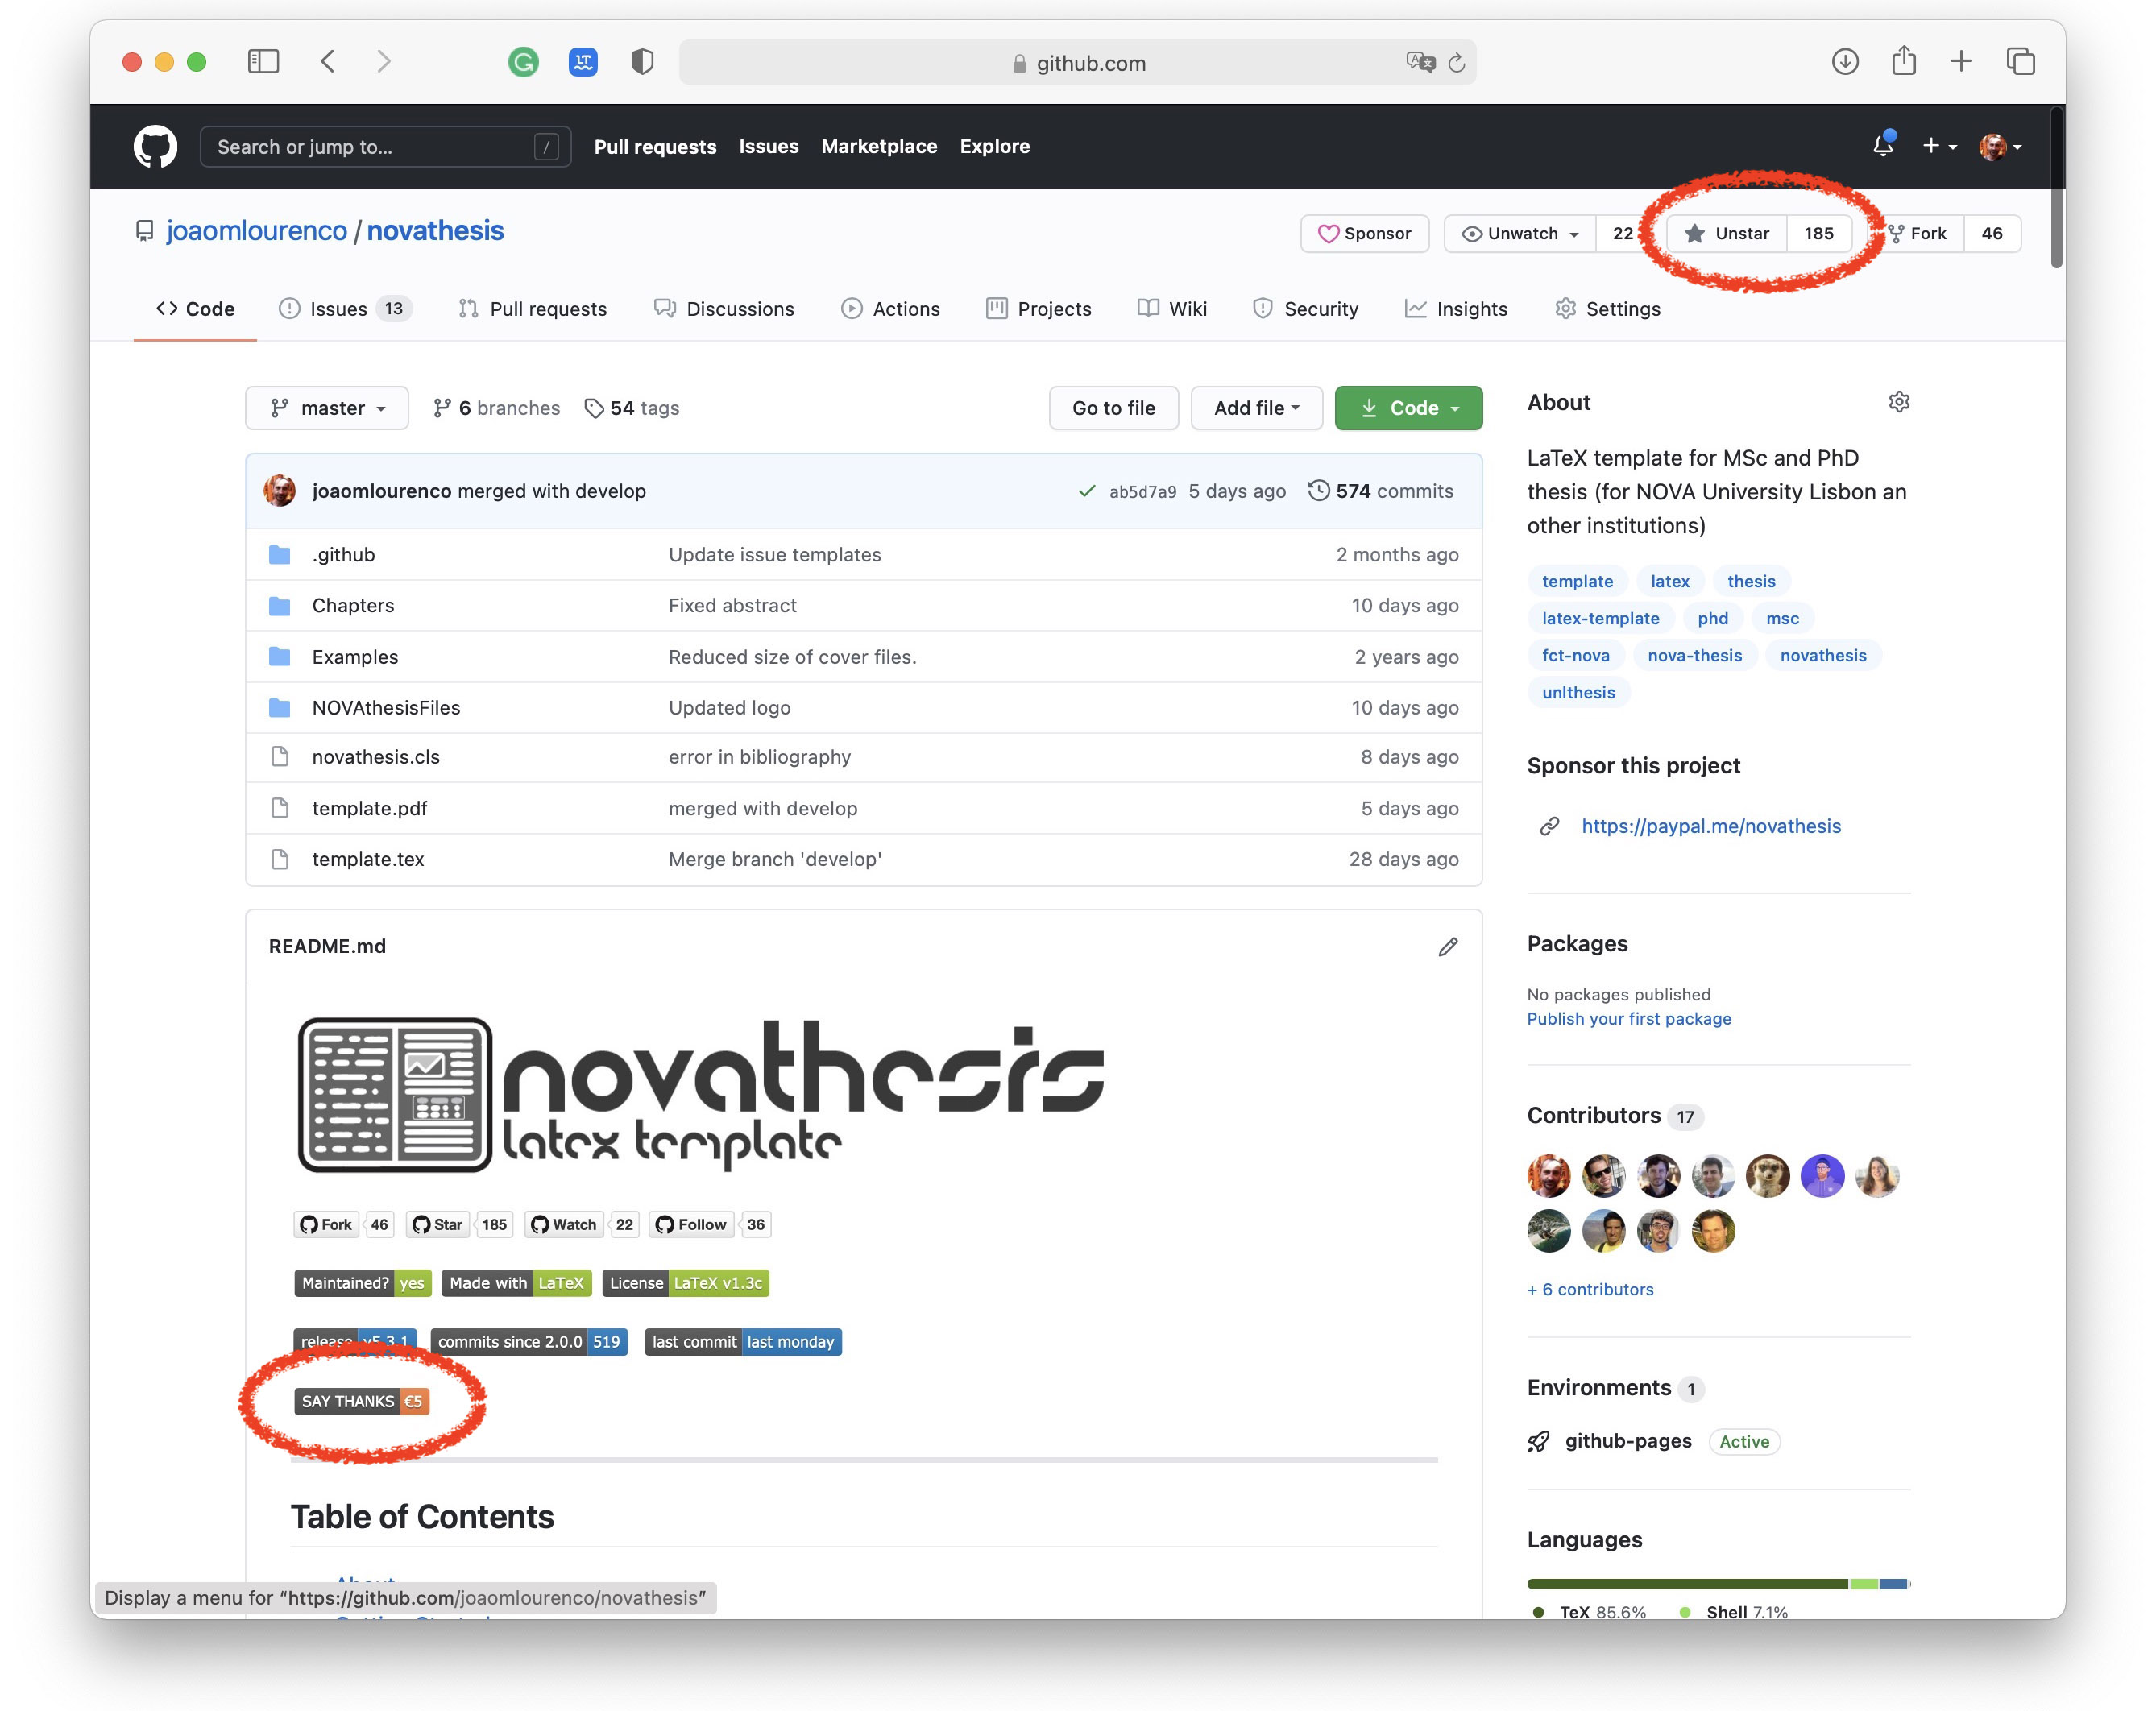
\includegraphics[width=0.5\linewidth]{github1}
    \caption{The \gls{novathesis} project web page in GitHub.}
    \label{fig:github}
\end{figure}

\section{The \emph{NOVAthesis} Template}
\label{sec:a_bit_of_history}

\ntindex[Template]{}

Tdfsdf



The \gls{novathesis} template exists to make your life easier and we do our best to make it compliant to the supported ($+25$) Schools' regulations but, in the end of the line, you and only you are accountable for both the look and the contents of the document you submit as your thesis/dissertation.
